\section{Recurrent Neural Networks (RNNs)}

\begin{frame}\frametitle{\subsecname}

\begin{itemize}
\item Feedforward netwroks:\\

\underline{Data}:
\begin{equation*}
\Big\{ \left(\vec x^{(\alpha)}, \vec y^{(\alpha)}_{\mathrm{True}} \right) \Big\}\,,\quad \alpha = 1,\ldots,p
\end{equation*}

\pause

\begin{itemize}
\item any two sample pairs $\left(\vec x^{(\alpha)}, \vec y^{(\alpha)}_{\mathrm{True}} \right)$ and $\left(\vec x^{(\alpha')}, \vec y^{(\alpha')}_{\mathrm{True}} \right)$ are assumed to be \iid
\item Their respective predictions $\vec y(\vec x^{(\alpha)}; \vec w)$ and $\vec y(\vec x^{(\alpha')}; \vec w)$ are also independent from one another.
\end{itemize}

\pause

\item RNN \corresponds~Neural network with loops.\\

\underline{Data}:\\

\begin{equation*}
\Big\{ \left(\vec x^{(\alpha,t)}, \vec y^{(\alpha,t)}_{\mathrm{True}} \right)_{t=1}^{n_{\alpha}} \Big\}\,,\quad \alpha = 1,\ldots,p
\end{equation*}

\pause

\begin{itemize}
\item $p$ \iid sequences
\item each sequence $\alpha$ contains $n_{\alpha}$ time steps
\item Use information from the previous step to predict the next step.
\end{itemize}

\end{itemize}

\end{frame}


\subsection{Basic RNN}


\begin{frame}\frametitle{\subsecname}

\begin{figure}[ht]
     \centering
	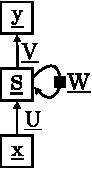
\includegraphics[width=0.2\textwidth]{img/rnn}
     \mode<article>{
	\caption{Basic RNN architecture}
	}
	\label{fig:rnn} 
\end{figure}
\end{frame}

\begin{frame}\frametitle{\subsecname}

%Omitting sequence index $\alpha$
\begin{figure}[ht]
     \centering
	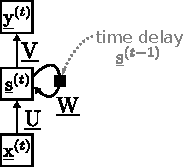
\includegraphics[width=0.4\textwidth]{img/rnn_time_delay}
     \mode<article>{
	\caption{Basic RNN architecture}
	}
	\label{fig:rnn} 
\end{figure}


\end{frame}

\subsubsection{Measure the activities}

\definecolor{darkgreen}{rgb}{0,0.6,0}

\begin{frame}\frametitle{\subsubsecname}

\mode<article>{
\begin{figure}[ht]
     \centering
	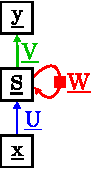
\includegraphics[width=0.2\textwidth]{img/rnn_colored}
     \mode<article>{
	\caption{Basic RNN architecture}
	}
	\label{fig:rnn} 
\end{figure}
}
\mode<presentation>{
\placeimage{13}{1}{img/rnn_colored}{width=2cm}
}

Let
\begin{itemize}
\item[] $N$ be the number of input variables $\rightarrow$ $\vec x^{(t)} \in \R^N$
\item[] $H$ be the number of hidden nodes
\item[] $M$ be the number of output nodes
\end{itemize}

\pause

Identify the free parameters (trainable weights) of the network:

\begin{itemize}
\item input-to-hidden: ${\color{blue} \vec U = (\vec u_1,\ldots, \vec u_i, \ldots,\vec u_H)} \in \R^{H,N}$
\item hidden-to-hidden: ${\color{red} \vec W = (\vec w_1,\ldots, \vec w_j, \ldots,\vec u_H)} \in \R^{H,H}$
\item hidden-to-output: ${\color{darkgreen} \vec V = (\vec v_1,\ldots, \vec v_k, \ldots,\vec v_H)} \in \R^{H,H}$
\end{itemize}




\end{frame}


% ------------------------------------------------------------------------------
\begin{frame}\frametitle{A simple RNN}
	\begin{minipage}{\textwidth}
		\begin{minipage}{0.21\textwidth}
			{\includegraphics<1>[width=\textwidth]{img/rnn_no_supscript.pdf}}
			{\includegraphics<2>[width=\textwidth]{img/rnn_no_supscript.pdf}}
			{\includegraphics<3>[width=\textwidth]{img/rnn_supscript.pdf}}
		\end{minipage}	
		\hspace{0.6cm}
		\begin{minipage}{0.6\textwidth}
		
		\begin{textblock}{10}(5.0,3.5)
			\only<1> {\small define $h_i^{(t)}$ and $y_k^{(t)}$:}
			\only<2> {\small switch from element-wise notation to vector notation}
			\only<3> {\small add superscripts to the different weight matrices}
		\end{textblock}
			\begin{eqnarray*}
			\only<1>{
				h_i^{(t)} &=& \tanh \Big({\smallsum{k=1}{N} U_{ik} \, x_k^{(t)}} 
						{ + \smallsum{j=1}{H}  W_{ij} \, h_j^{(t-1)}}
						+ b^h_i \Big) \,,
						\\
				y_k^{(t)} &=& f\Big({\smallsum{j=1}{H} 
						V_{kj} \, h_j^{(t)}} + b^y_k\Big) \,,\\[0.7cm]
					\;\text{e.g.}\;f(\cdot) &:=& \mathrm{ softmax}(\cdot)\\
					}
			\only<2>{
				\vec h^{(t)} &=& \tanh\Big({\vec U \, \vec x^{(t)}} 
						{ + vec W \, \vec h^{(t-1)}}
						+ \vec b^h \Big) \,,
						\\
				\vec y^{(t)} &=& f\Big({\vec V \, h^{(t)}} + \vec b^y\Big) \,,\\[0.7cm]
					\;\text{e.g.}\;f(\cdot) &:=& \mathrm{softmax}(\cdot)\\
					}
			\only<3>{
				\vec h^{(t)} &=& \tanh\Big({\vec U^h \, \vec x^{(t)}} 
						{ + \vec W^h \, \vec h^{(t-1)}}
						+ \vec b^h \Big) \,,
						\\
				\vec y^{(t)} &=& f\Big({\vec V^h \, \vec h^{(t)}} + \vec b^y\Big) \,,\\[0.7cm]
					\;\text{e.g.}\;f(\cdot) &:=& \mathrm{softmax}(\cdot)\\
					}
			\end{eqnarray*}
		\end{minipage}
	\end{minipage}
\end{frame}
